\section{Layout}

%---------------------------------------------------------------------------------
\begin{frame}[fragile]
\frametitle{Layout}
\color{structure}
Rendering
\begin{itemize}\color{structure}
\item the rendering is controlled by
\begin{itemize}
  \item element tag: \html{<p>, <select>}
  \item properties: \html{font-family, background-color}
\end{itemize} 
\item some properties are dynamic, updated by the browser rendering engine
\item most properties are inherited from the surrounding
\item properties can not be deleted, only shadowed
\item give an property a value:
\begin{itemize}\color{structure}
  \item the \html{style} attributet in the HTML element
  \item Cascading Style Sheets (CSS)
  \end{itemize}
\end{itemize}

\bigskip
\href{https://www.w3schools.com/css/css_intro.asp}{example of what you can do with css: https://www.w3schools.com/css/css\_intro.asp}
\end{frame}

%---------------------------------------------------------------------------------
\begin{frame}[fragile]
\frametitle{CSS}
\color{structure}
Cascading Style Sheets
\begin{itemize}\color{structure}
\item separate the content from the layout
\item a set of rules:
\begin{itemize}\color{structure}
  \item  selection
  \item declaration (attribut = value)
\end{itemize}
\item the declaration is applied to all elements matching the selection
\end{itemize}
syntax:\\ \code{urval : \{ property1: value1; property2: value2;\}}
\end{frame}

%---------------------------------------------------------------------------------
\begin{frame}[fragile]
\frametitle{CSS - selection}
\color{structure}
CSS selection is based on pattern matching:\\
\begin{itemize}\color{structure}
\item instances of an element: \html{<h1>}
\item all elements with a class: \html{<div class="my-style">}
\item the element with a given \tt{id}: \html{<div id="my-tag">}
\item pseudo classes \html{focus, hover, visited, valid, ...}
\item pseudo element \html{nth-child(2), only-child, ...} 
\item attribute value: \html{[title~="flower"], ...} 
\end{itemize}
Match patterns can be combined
\end{frame}

%---------------------------------------------------------------------------------
\begin{frame}[fragile]
\frametitle{CSS - exempel}
\color{structure}
Example:
\begin{lstlisting}[style=htmlcssjs]
// element
div { color: blue; border: 1px; }
// id, <p id="my-blue-box">
#my-blue-box { background-color: lightblue; }
// class, <div class="center">
.center { text-align: center; color: red; }
// element och and, <p class="center">
p.center { text-align: center; color: green; }
// inside
div p { text-align: center; color: green; }
// all p with a parent div
div > p { text-align: center; color: green; }
// directly after
div + p { text-align: center; color: green; }
// pseudo-class
a:hover { background-color: lightblue; }
\end{lstlisting}
\end{frame}

%---------------------------------------------------------------------------------
\begin{frame}[fragile]
\frametitle{Box Modellen}
\color{structure}
  \centering
  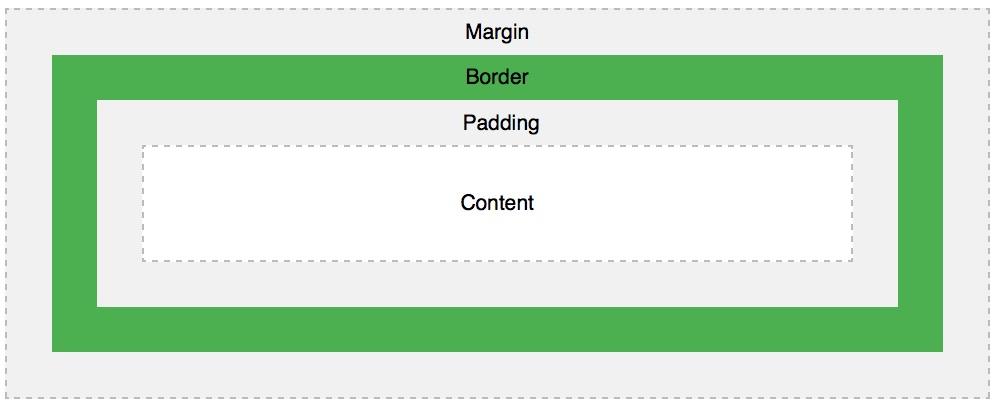
\includegraphics[width=10cm]{img/box_model}

\end{frame}

%---------------------------------------------------------------------------------
\begin{frame}[fragile]
\frametitle{Layout}
\color{structure}
CSS Properties for layout
\begin{itemize}
  \item \code{display}: \code{block, inline, none, flex, ...}
  \item \code{visibility}: \code{visible, hidden, ...}
  \item \code{position}: \code{static, relative, absolute, fixed, ...}
  \item \code{overflow}: \code{visible, hidden, scroll, auto, ...}
  \item \code{z-index}: \code{auto}, \it{number}
\end{itemize}
\end{frame}

%---------------------------------------------------------------------------------
\begin{frame}[fragile]
\frametitle{Frameworks}
\color{structure}
Creating a good layout is costly. 
\begin{itemize}\color{structure}
  \item needs a lot of testing on different browsers
  \item you can use or extend use existing:
  \begin{itemize}
    \item bootstrap
    \item material design
  \end{itemize}
\end{itemize}
\end{frame}

%---------------------------------------------------------------------------------
\begin{frame}[fragile]
\frametitle{My own standard}
\color{structure}
Each browser have their own implementation of the
\begin{itemize}\color{structure}
  \item rendering engine
  \item JavaScript engine
\end{itemize}
\vspace{5mm}
With their own
\begin{itemize}\color{structure}
  \item interpretation of the standard
  \item selection of standard features to support
  \item bugs
  \item extensions
\end{itemize}
\end{frame}

%---------------------------------------------------------------------------------
\begin{frame}[fragile]
\frametitle{Webkit Mozilla}
\color{structure}
The same feature apperas with different names in different browsers:
\begin{itemize}\color{structure}
  \item \code{box-shadow}
  \item \code{-webkit-box-shadow}
  \item \code{-moz-box-shadow}
\end{itemize}
\end{frame}

